\maketitle

\section{Descripcion del Problema}
El comedor universitario atiende estudiantes universitarios que requieren
alimentarse. El problema fundamental es que actualmente el sistema no ofrece
satisfacción a sus usuarios porque los cupos son insuficientes. Hay 3,000
cupos, los cuales no satisfacen la demanda para 20,000 estudiantes. Es
necesario desarrollar una solución transparente de distribución de cupos.

\section{Planificacion del Proyecto}
\subsection{Planificacion de Iteraciones}
\noindent\textbf{Epicas}\par
\begin{enumerate}
    \item Como miembro del Equipo de desarrollo del proyecto COMEDOR
        UNIVERSITARIO, quiero definir las herramientas que voy a utilizar y
        configurar mi ambiente de trabajo para trabajar en el proyecto.
    \item Como administrador del Comedor Universitario, quiero contar con la
        base de datos de alumnos de los ciclos 5, 6 y 7 de Ingeniería
        Informática, para tener una base de datos de prueba alumnos usuarios
        del Comedor Universitario.
    \item Como Administrador del Comedor Universitario, quiero asignar cupos a
        un determinado número de comensales para brindarles el servicio de
        alimentación diaria (De lunes a viernes)
    \item Como Administrador del Comedor Universitario, quiero cobrar derechos
        de atención a los comensales, para financiar una parte del costo de
        atención a los COMENSALES
    \item Como Administrador del Comedor Universitario, quiero ATENDER a los
        que recibieron un cupo de atención en el COMEDOR UNIVERSITARIO
    \item Como Administrador del Comedor Universitario, quiero saber las
        frecuencias de uso del Comedor Universitario, para analizar el
        comportamiento de mis usuarios del Comedor
\end{enumerate}

\noindent\textbf{Historias de Usuario y Tareas}\par
TODO: hacer esta wea
% \begin{table}[h]
%     \begin{center}
%         \begin{tabular}[c]{l|m{3cm}|l|l}
%             \hline
%             \multicolumn{1}{c|}{\textbf{Epica}} &
%             \multicolumn{1}{c|}{\textbf{Historia de Usuario}} &
%             \multicolumn{1}{c|}{\textbf{Costo}} &
%             \multicolumn{1}{c}{\textbf{Encargado}} \\
%             \hline
%             Epica & Historia de Usuario & Costo & Encargado(s)\\
Epica & Historia de Usuario & Costo & Encargado(s)\\
Epica & Historia de Usuario & Costo & Encargado(s)\\
Epica & Historia de Usuario & Costo & Encargado(s)\\
Epica & Historia de Usuario & Costo & Encargado(s)\\
Epica & Historia de Usuario & Costo & Encargado(s)\\
Epica & Historia de Usuario & Costo & Encargado(s)\\
 \\
%             \hline
%         \end{tabular}
%     \end{center}
% \end{table}


\newpage
\subsection{Planificacion del Trabajo}
\noindent\textbf{Distribucion de Roles}\par
\begin{table}[h]
    \begin{tabular}{|l|c|}
        \hline
        Rol & Encargado \\
        \hline
        Scrum Master & Johan Conde \\
        Project Owner & Ludvika Ccasa \\
        Frontend Developer & Alain Condori \\
        Backend Developer & Alex Berrios \\
        UX/UI Designer & Daniel Alegria \\
        \hline
    \end{tabular}
\end{table}

\noindent\textbf{Horario}\par
Se utilizara la herramienta \textit{Google Meet} en el cual usaremos un canal
para que el gerente del trabajo pueda supervisar la reunion. Se haran:
\begin{itemize}
    \item 3 reuniones a la semana de max 10 min.
    \item 1 reunion de 1 hora para la Planificacion de Iteracion
\end{itemize}

%%%%%%%%%%%%%%%%%%%%%%{CALENDAR}%%%%%%%%%%%%%%%%%%%%%%%%%%%
\newpage
Las planificaciones de la iteracion se llevaran a las 6pm y las reuniones
breves de 10 minutos se realizaran a las 10pm en las fechas acordadas que se
indica a continuacion. El calendario de actividades cuenta con los siguientes
elementos:

\begin{figure}[h]
    \hspace{1cm}
    \fbox{ 
\includegraphics[width=0.5\textwidth]{images/cal_legend.png} }
\end{figure}

\begin{figure}[h]
    \fbox{ 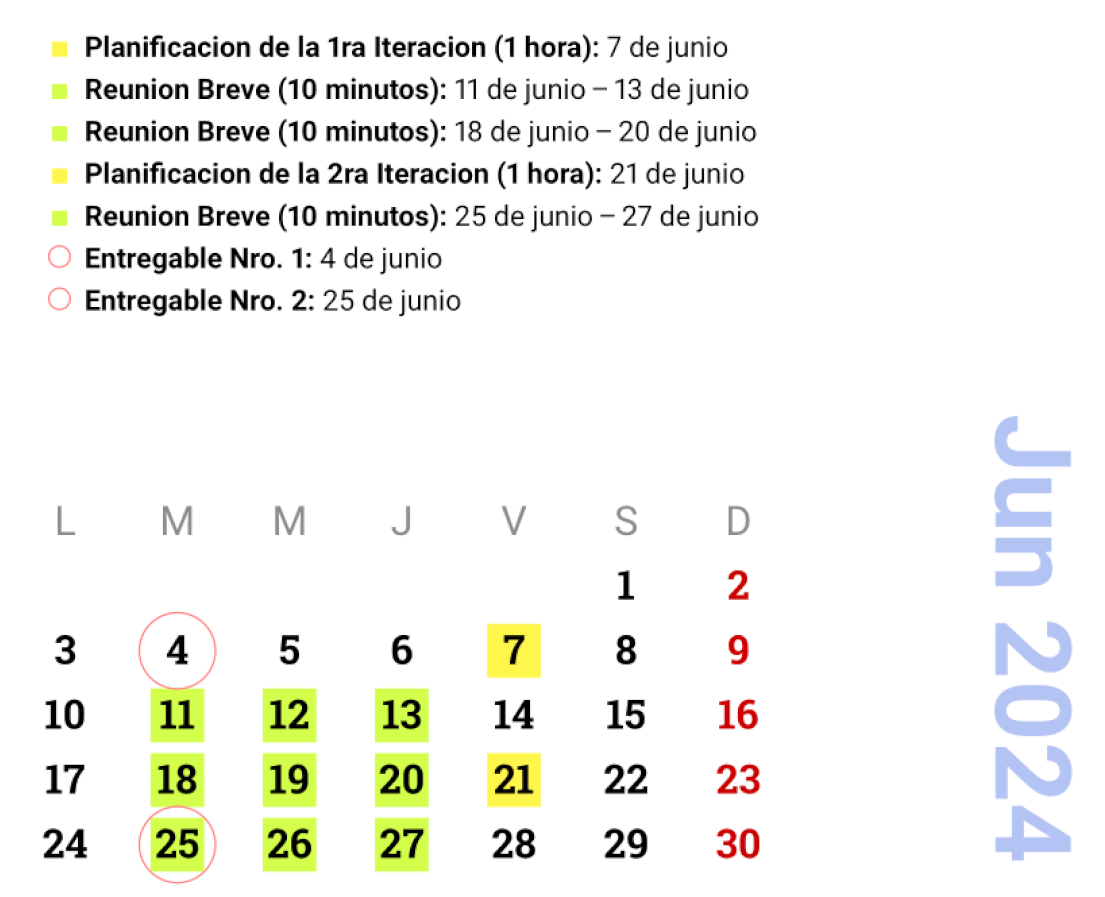
\includegraphics[width=0.5\textwidth]{images/cal_junio.png} }
    \fbox{ 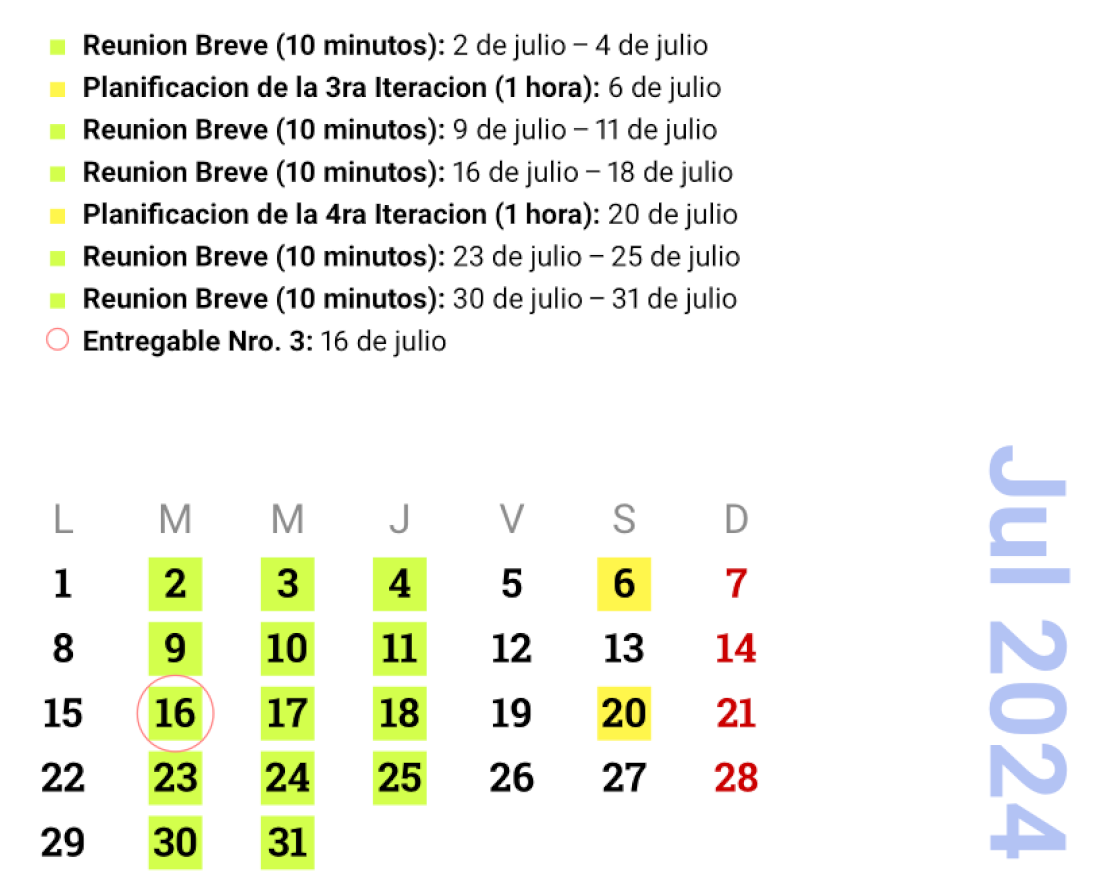
\includegraphics[width=0.5\textwidth]{images/cal_julio.png} }
    \fbox{ 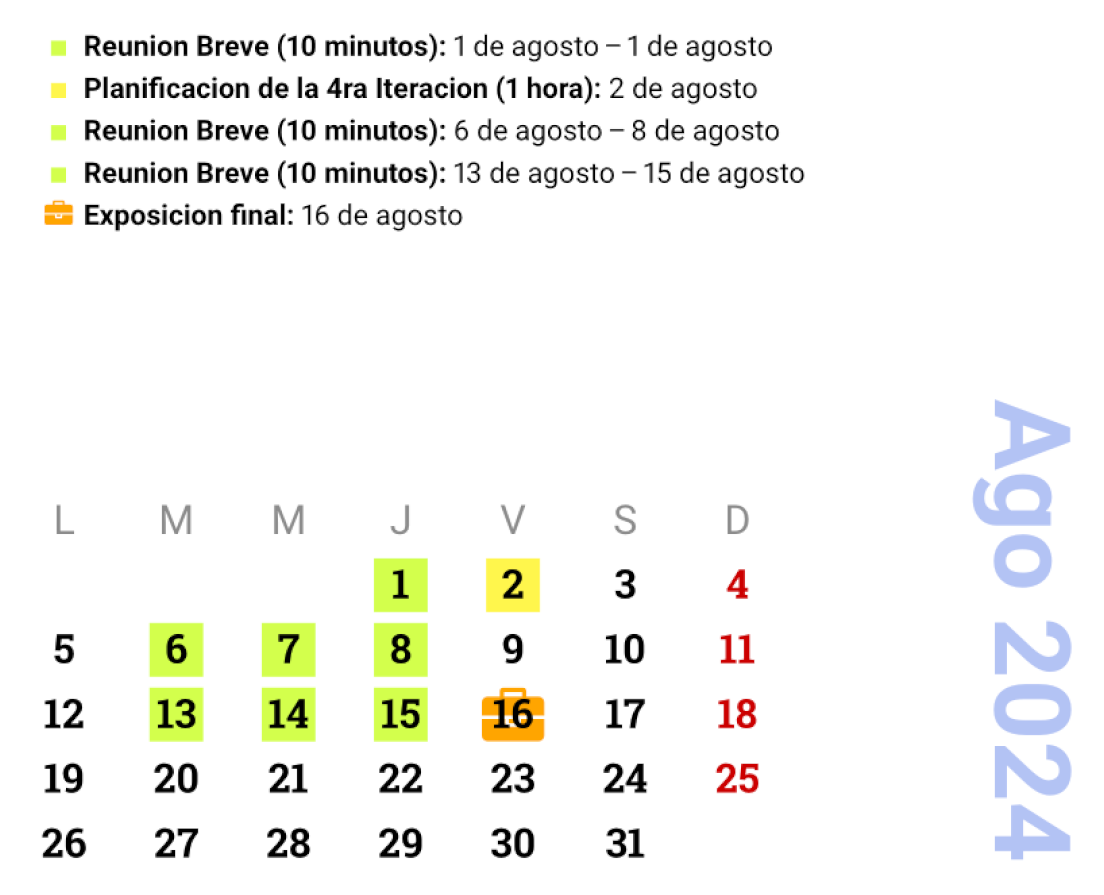
\includegraphics[width=0.5\textwidth]{images/cal_agosto.png} }
\end{figure}

%%%%%%%%%%%%%%%%%%%%%%%%%%%%%%%%%%%%%%%%%%%%%%%%%%%%%%%%%%%
\newpage
\subsection{Azure Devops}

\noindent\textbf{Uso de azure Devops}
\begin{figure}[h]
    \caption{Johan Conde}
    \begin{center}
        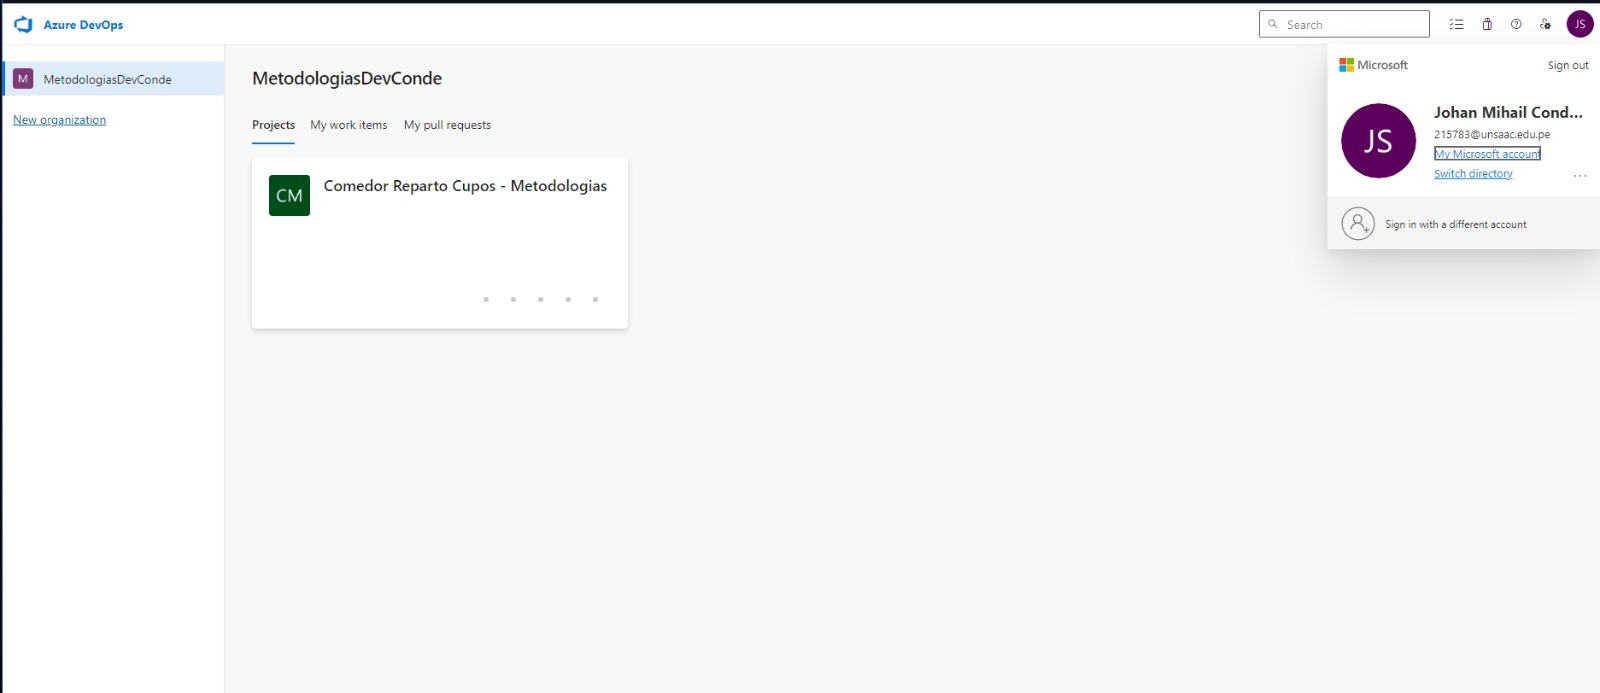
\includegraphics[width=0.95\textwidth]{images/devops_conde.jpeg}
    \end{center}
\end{figure}

\begin{figure}[h]
    \caption{Ludvika Ccasa}
    \begin{center}
        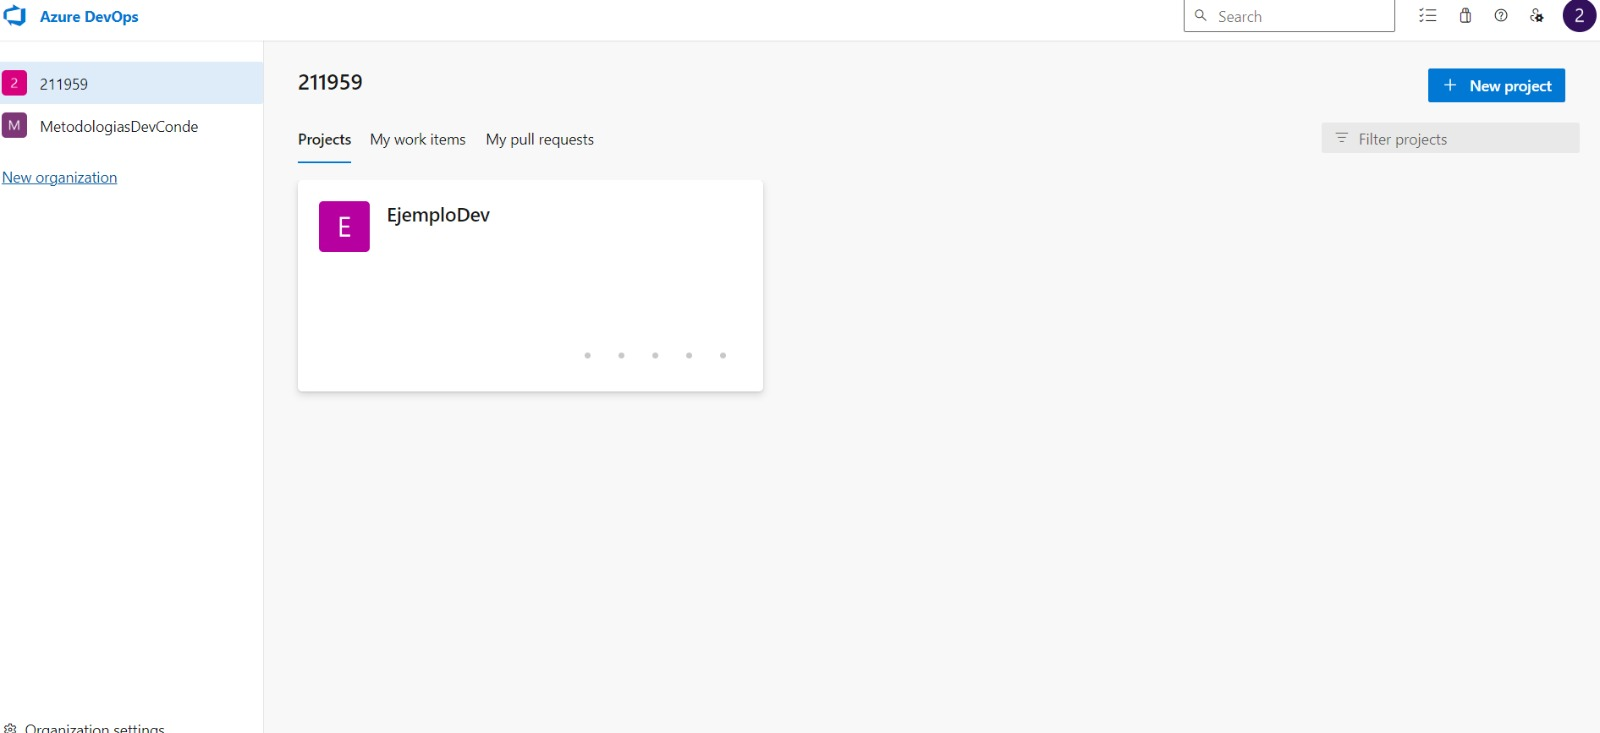
\includegraphics[width=0.95\textwidth]{images/devops_ccasa.jpeg}
    \end{center}
\end{figure}

\begin{figure}[h]
    \caption{Alain Condori}
    \begin{center}
        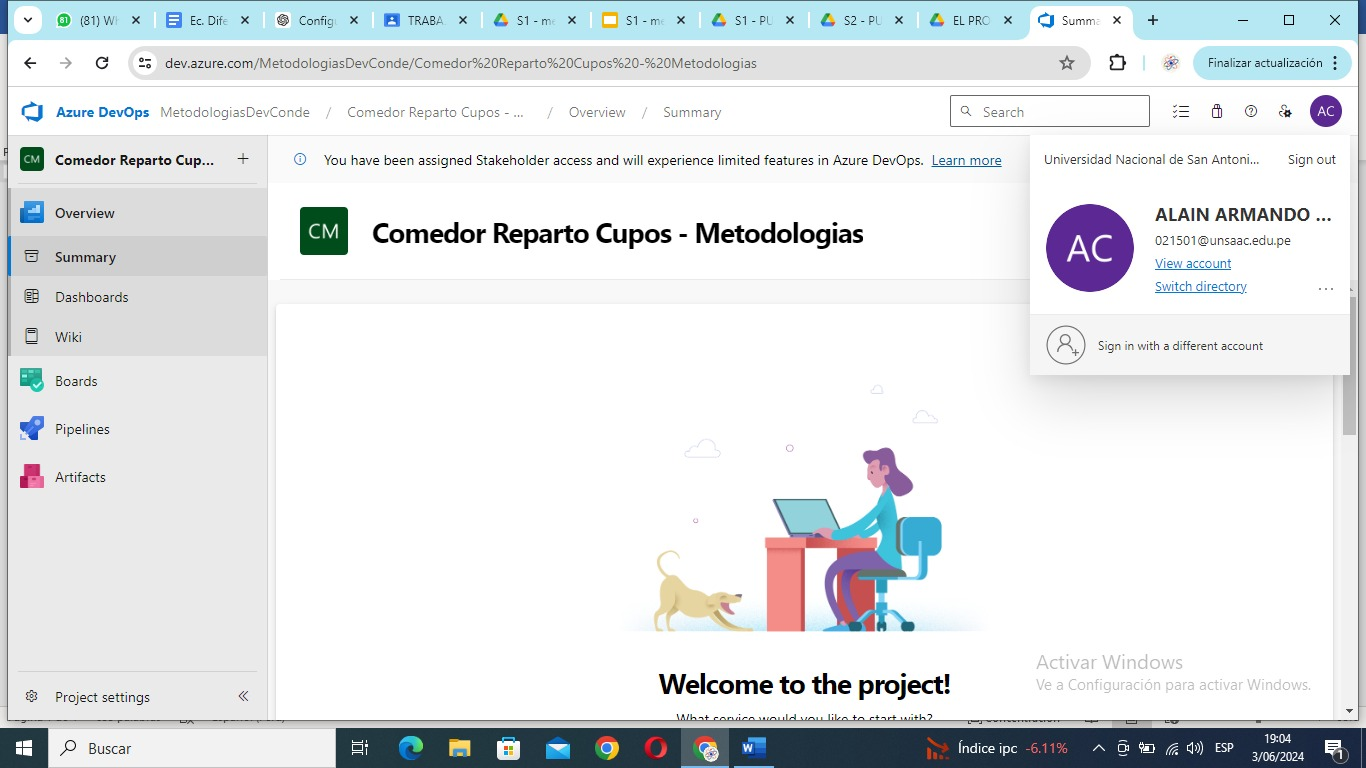
\includegraphics[width=0.95\textwidth]{images/devops_condori.jpeg}
    \end{center}
\end{figure}

\begin{figure}[h]
    \caption{Alex Berrios}
    \begin{center}
        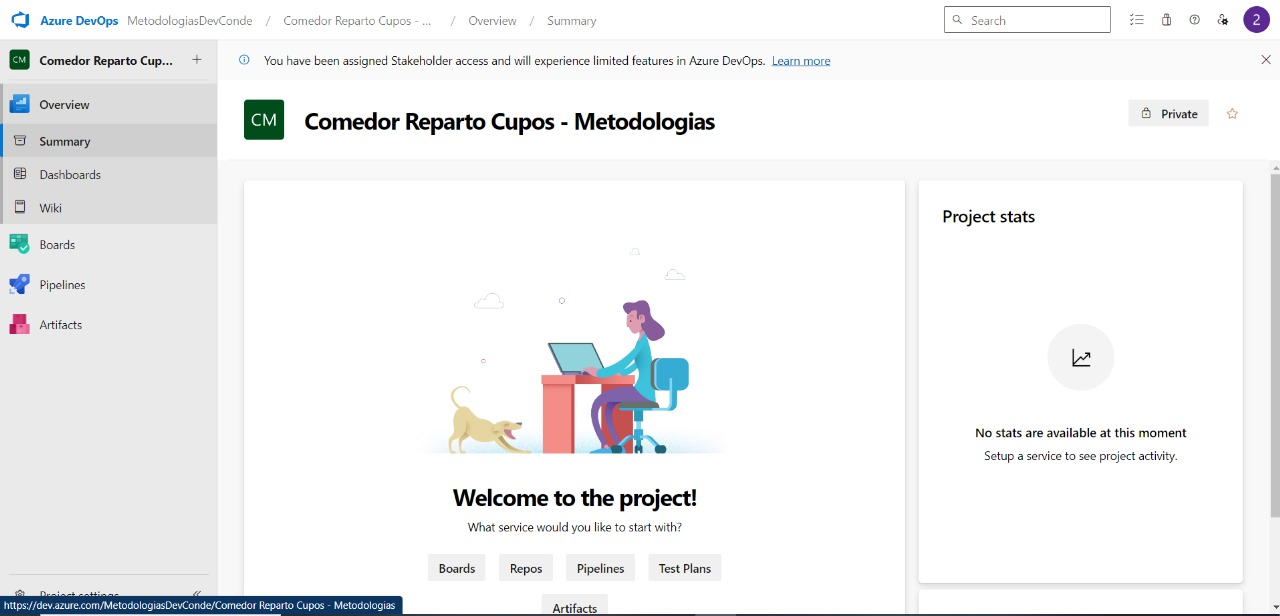
\includegraphics[width=0.95\textwidth]{images/devops_berrios.jpeg}
    \end{center}
\end{figure}

\begin{figure}[h]
    \caption{Daniel Alegria}
    \begin{center}
        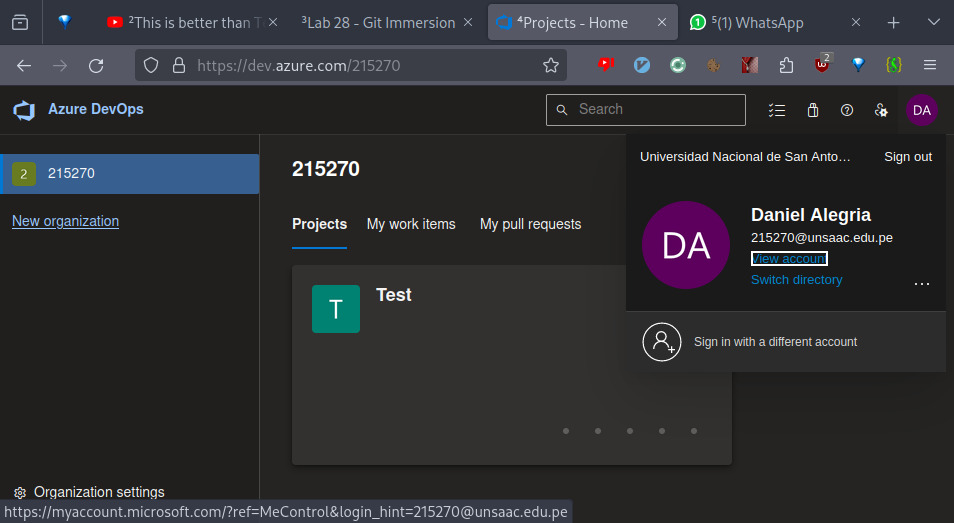
\includegraphics[width=0.95\textwidth]{images/devops_alegria.jpeg}
    \end{center}
\end{figure}

